\chapter{Omisión de palabras}


Los capítulos anteriores se han enfocado en tratar a las migraciones de palabras como fenómenos consecuentes de eventos las lenguas están involucradas. Un punto clave para llegar en el proceso fue clasificar a los $n$-grams en palabras funcionales y palabras de contenido, y a partir de dicha clasificación restringir de la base de datos a a las palabras funcionales, es decir artículos, preposiciones, conjunciones y pronombres. En principio  las palabras funcionales son las más utilizadas en los idiomas, independientemente del idioma que se este tratando \cite{iplosone}, no obstante  el significado que conllevan no ayuda a hacer relaciones con los eventos. 

El realizar la omisión anterior permitió encontrar algunos resultados acordes a la relación evento-migración, pero ¿qué sucedería si en los idiomas se hicieran otras restricciones para excluir un grupo determinado de palabras? , ¿de qué manera afectaría esta limitación a las migraciones y al uso de un idioma en otro?

Estas interrogantes han llevado a la construcción de un nuevo algoritmo que limite a las palabras, reduzca el conjunto de las migraciones y obtenga nuevos valores del uso entre idiomas. Escogidos una pareja de idioma origen \textit{A} e idioma receptor \textit{B}, el proceso es el siguiente. 


\begin{enumerate}
	
	\item Se toma la lista de los préstamos acumulados de \textit{A} en \textit{B},  este conjunto se denotará como \textbf{conjunto original}.
		
	\item Se escogen de forma aleatoria un conjunto de letras (desde una hasta cuatro), y se eliminaran de los préstamos acumulados a todas las palabras cuya primer letra sea alguna de las elegidas. Este nuevo grupo se puntualiza como \textbf{conjunto reducido}.
	
	\item Se establece un tercer cúmulo designado como \textbf{conjunto residuo} conformado por todas las palabras que se han eliminado del conjunto original.  Cabe decir que la unión del reducido y el residuo dan como resultado el original. 
	
	\item En los tres conjuntos se empleó la ecuación \ref{ec.fuso}, para encontrar el uso de \textit{A} en \textit{B}. 	
	 
\end{enumerate}

Tras la descripción, las primeras dudas que surge es el por qué limitar las eliminaciones a aquellas palabras que empiecen con una determinada letra,  y por qué solo tomar cuatro letras de todas las posibles del abecedario.  La razón  de la primera cuestión  se basa en que es la manera más sencilla de eliminar un grupo de palabras; referente a la cantidad de letras se hicieron las exclusiones hasta para diez letras,  sin embargo para algunas combinaciones de idiomas y elecciones de mas de seis letras, el conjunto reducido no contenía elementos, siendo el residuo igual al original. La intención de estas alteraciones no es desaparecer el conjunto de las migraciones sino el reducirlas y estudiar en ellas que tanto cambia el uso. 

Una forma para comprender la variación del uso entre los conjuntos original y residuo es a través del coeficiente de determinación; en el próximo capítulo se abordara más en su formalismo. La primera pauta a seguir será al tomar el uso en el conjunto original como verdadero (ya que con el se establecieron los resultados del capítulo anterior) identificando sus valores a lo largo del tiempo $t$ con la variable $O(t)$, si los valores de uso en el conjunto reducido se denotan como  $v(t)$ y el promedio de ellos es $\bar{v}$, entonces   el coeficiente de determinación queda definido como :
 
\begin{equation}
 \label{ec.dif_uso}
 R^{2} = 1 - \sum_{t} \frac{ \left( v(t)- O(t) \right)^{2}  }{ \left( v(t) - \bar{v} \right)^{2} }
\end{equation}

Se define el concepto \textbf{conservación del uso} para aquellos pares de conjuntos donde el uso no cambie a pesar de las omisiones. Su aserto  recaerá en los valores de $R^{2}$ próximos a 1,  indicando que el uso se conserva, en consecuencia las omisiones no afectaron a los conjuntos, en caso contrario $R^{2}$ tomará valores cercanos a cero.

Para la presentación de resultados, se graficó en color negro los valores de uso en el conjunto original, sin importar que combinación de idiomas se este tratando.  Para el conjunto reducido, el uso se marcó en color rojo.  En cada grafica se especifica que letras se usaron para las reducciones. 

\newpage

\subsubsection*{Inglés}

\begin{figure}[h!]
	\centering
	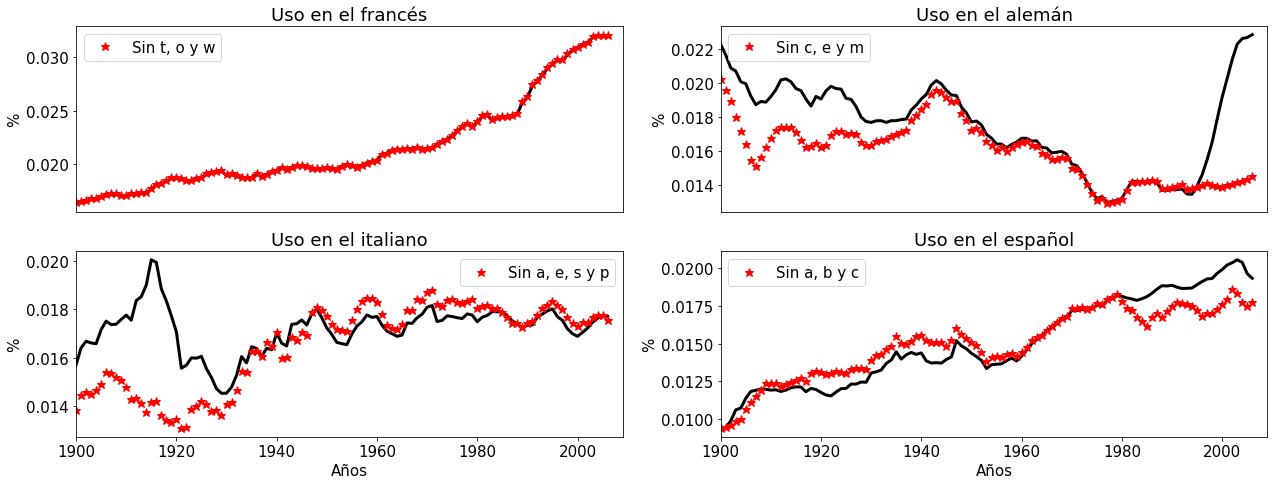
\includegraphics[width=14.5cm, height=6.8cm]{OM_EN.png}
	\label{fig.OM_EN}
	\caption{Omisiones del inglés.}
\end{figure}


\subsubsection*{Francés}

\begin{figure}[h!]
	\centering
	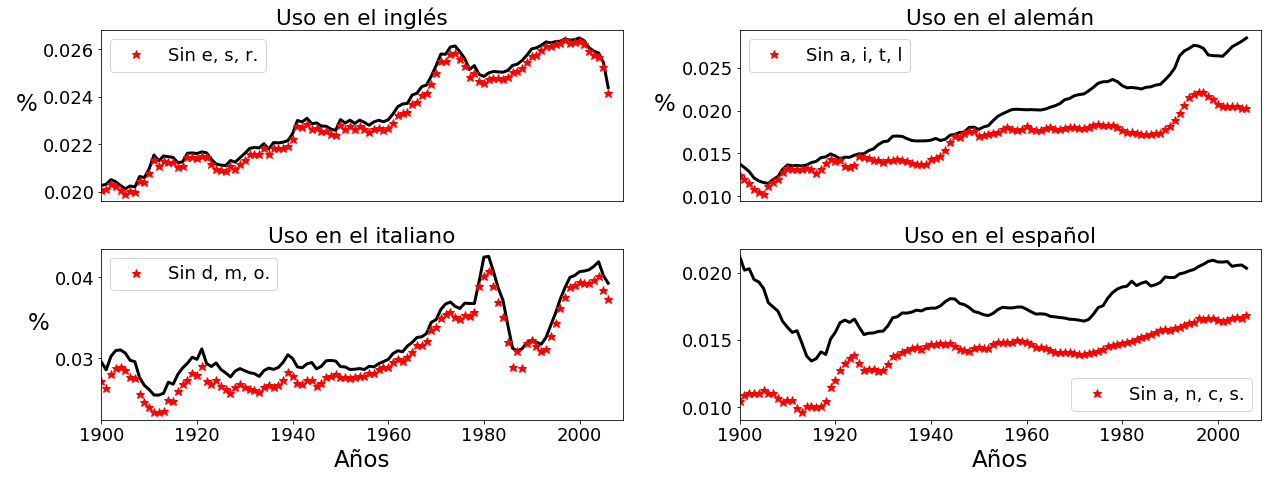
\includegraphics[width=14.5cm, height=6.8cm]{OM_FR.png}
	\label{fig.OM_FR}
	\caption{Omisiones del francés.}
\end{figure}


\newpage
\subsubsection*{Alemán}

\begin{figure}[h!]
	\centering
	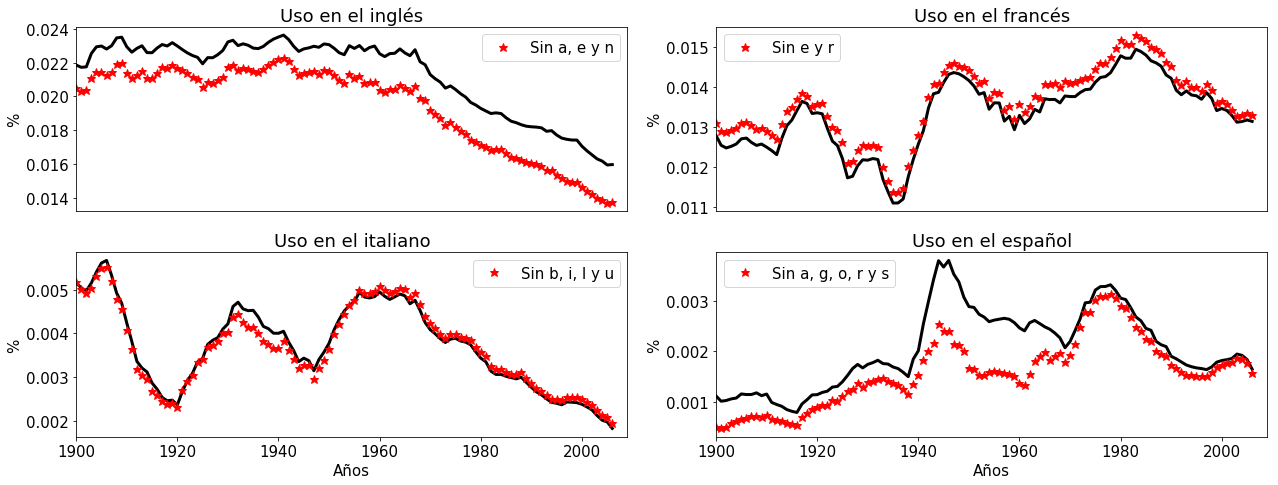
\includegraphics[width=14.5cm, height=6.8cm]{OM_GE.png}
	\label{fig.OM_GE}
	\caption{Omisiones del alemán.}
\end{figure}


\subsubsection*{Italiano}

\begin{figure}[h!]
	\centering
	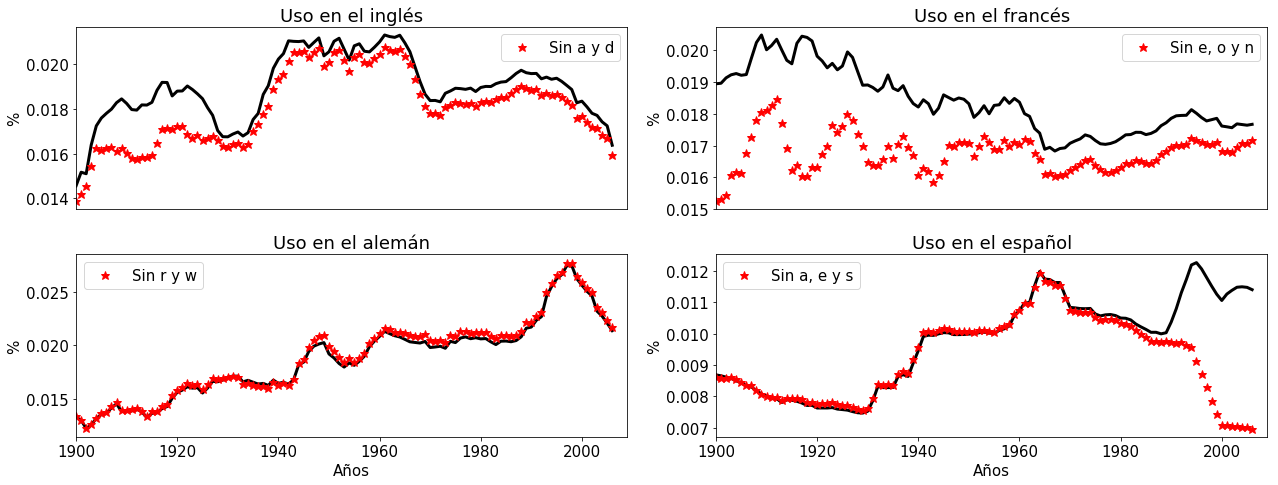
\includegraphics[width=14.5cm, height=6.8cm]{OM_IT.png}
	\label{fig.OM_IT}
	\caption{Omisiones del italiano.}
\end{figure}

\newpage
\subsubsection*{Español}

\begin{figure}[h!]
	\centering
	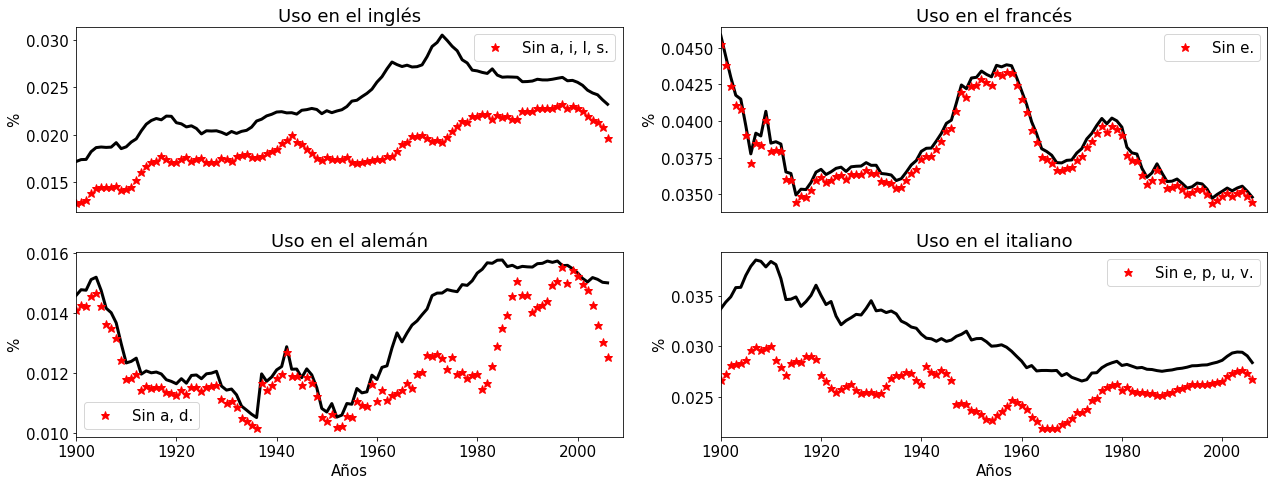
\includegraphics[width=14cm, height=6.8cm]{OM_SP.png}
	\label{fig.OM_SP}
	\caption{Omisiones del español.}
\end{figure}


Tras reducir el corpus de palabras con diferentes condiciones, se distinguieron las siguientes características en el comportamiento de un idioma en otro:


\begin{itemize}
	
	\item Valores iguales. Punto a punto el conjunto reducido empalma al original, siendo las gráficas indistinguibles, indicando conservacion del uso. 
		
	\item Diferencia de alturas. Ambas gráficas muestran el mismo comportamiento en la escala de tiempo, sin embargo existe  una diferencia constante entre el uso original y el reducido. En este caso se dirá que el uso también se conserva ya que ambas graficas tienen los mismos valores sólo que están desfasados. 
	
	\item Diferencias por periodos. Una combinación de los puntos anteriores,  donde las graficas son idénticas salvo en algún periodo donde se presenta la diferencia de alturas. La conservación se da por periodos de tiempo menos prolongados. 
	
	\item Alteraciones prolongadas. Se caracteriza por periodos donde ambos valores de uso son completamente diferentes.  El uso al no conservarse indicara que los préstamos omitidos son los más relevantes en estas etapas. 
			
\end{itemize}


La elección de las letras que se utilizaron para realizar las graficas fueron completamente aleatorias; el que una combinación presente alguna de las características mencionadas no significa que sea la misma para otras alternativas que puedan deformar más o menos e incluso desaparecer el conjunto reducido.  

Para sostener la conservación del uso tratada en las características mencionadas,  se calculó en cada punto la diferencia de alturas entre ambos valores y con ello su valor promedio $\Delta h$; esta cifra se aumentó en todos los valores reducidos $v(t)$ con la intención de que coincidieran lo más posible con los originales $U(t)$, asi el valor de $R^{2}$ es más adecuado.

\fxwarning{Pongo la tabla para notar los valores de R2 y ver por un valor la similitud,  a mi gusto seria bueno poner que tanto cambiaron los conjuntos al hacer las eliminaciones, aunque si la tabla parece relleno por todas las combinaciones hechas, mejor eliminarla}


\begin{table}[h!]
	\centering
	\begin{tabular}{ccc}
		\textbf{}  & \textbf{$\Delta h$}  & \textbf{$R^{2}$}      \\
		\textbf{inglés-francés}    & 0.001           & 0.99       \\
		\textbf{inglés-alemán}     & 0.003           & 0.91       \\
		\textbf{ingles-italiano}   & 0.004           & 0.63       \\
		\textbf{ingles-español}    & 0.002           & 0.93       \\
		\textbf{francés-inglés}    & 0.001           & 0.98       \\    
		\textbf{francés-alemán}    & 0.003           & 0.84       \\ 
		\textbf{francés-italiano}  & 0.002           & 0.81       \\ 
		\textbf{francés-español}   & 0.003           & 0.81       \\ 
		\textbf{alemán-inglés}     & 0.002           & 0.98       \\
		\textbf{alemán-francés}    & 0.002           & 0.88       \\
		\textbf{alemán-italiano}   & 0.001           & 0.99       \\
		\textbf{alemán-español}    & 0.003           & 0.96       \\
		\textbf{italiano-inglés}   & 0.002           & 0.78       \\
		\textbf{italiano-francés}  & 0.003           & 0.79       \\
		\textbf{italiano-alemán}   & 0.001           & 0.97       \\
		\textbf{italiano-español}  & 0.002           & 0.89       \\
		\textbf{español-inglés}    & 0.004           & 0.85       \\
		\textbf{español-francés}   & 0.001           & 0.99       \\
		\textbf{español-alemán}    & 0.003           & 0.67       \\
		\textbf{español-italiano}  & 0.004           & 0.74       
	\end{tabular}
	\caption{Parámetros de las omisiones.}
	\label{tab.Omision}
\end{table}


A partir de la tabla, se muestra que la mejor similitud entre los conjuntos se da en aquellos donde no hay alteraciones prolongadas; como se menciono anteriormente el que se tenga esta característica entre dos idiomas depende de la elección de palabras que restringen al conjunto, alguna otra combinación modificara las características entre  el conjunto original y el reducido, sin embargo se comprobó con diferentes muestreos que los casos donde hay alteraciones prolongadas son escasos.


\section{Comentarios del método}

El realizar diferentes elecciones para restringir a las palabras que conforman los prestamos de un idioma en otro, mostró desde el punto de vista estadístico que no importan cuales elementos conforman el corpus, la propiedad del uso es la misma, ya que individualmente los valores de uso de una única palabra pueden variar en los años del análisis y ser distintos a los de otra palabra, sin embargo al tratar a todo el conjunto, el uso se comporta de la misma  manera, sin importar los valores individuales de los elementos que lo conforman. 







